% answers.tex —— 2005 年·普通高等学校招生考试·山东卷·文科 · 参考答案与详细解析片段
% 由 tools/generate_projects.py 依来源总账自 2005/2005_数学真题_山东文科_试题.md + 2005/2005_数学真题_山东文科_解析正文.md + 2005/2005_数学真题_山东文科_答案要点.md 生成，勿手改（改源 MD 后重跑）


\begin{gktip}
固定源 PDF 为印刷页码 260–261 的两页题面，不附官方答案。以下解析均依据固定源独立推导复算；各题配图在 LaTeX 工程中均以 TikZ 纯矢量重绘。
\end{gktip}

\begin{answer}
\gksolhead{1}{}

\textbf{题目}：

$\{a_n\}$ 是首项 $a_1 = 1$，公差 $d = 3$ 的等差数列，如果 $a_n = 2005$，则序号 $n$ 等于\mbox{（　　）}

\begin{gkopts}(4)
\task A．$667$
\task B．$668$
\task C．$669$
\task D．$670$
\end{gkopts}

\Needspace{4\baselineskip}
\textbf{解析}

等差数列 $\{a_n\}$ 的首项 $a_1 = 1$，公差 $d = 3$．
\Needspace{5\baselineskip}
其通项公式为：
\nopagebreak[4]
\[
a_n = a_1 + (n - 1)d = 1 + 3(n - 1) = 3n - 2.
\]
\Needspace{5\baselineskip}
已知 $a_n = 2005$，代入得：
\nopagebreak[4]
\[
3n - 2 = 2005 \implies 3n = 2007 \implies n = 669.
\]

故选 C．

\gkanswer{答案：C}

\end{answer}
\begin{answer}
\gksolhead{2}{}

\textbf{题目}：

下列大小关系正确的是\mbox{（　　）}

\begin{gkopts}(2)
\task A．$0.4^3 < 3^{0.4} < \log_4 0.3$
\task B．$0.4^3 < \log_4 0.3 < 3^{0.4}$
\task C．$\log_4 0.3 < 0.4^3 < 3^{0.4}$
\task D．$\log_4 0.3 < 3^{0.4} < 0.4^3$
\end{gkopts}

\Needspace{4\baselineskip}
\textbf{解析}

分别估计各数值的大小：
\Needspace{5\baselineskip}
1. 对数式：因为底数 $4 > 1$，真数 $0.3 \in (0, 1)$，所以
\nopagebreak[4]
\[
\log_4 0.3 < \log_4 1 = 0.
\]
\Needspace{5\baselineskip}
2. 指数式 $0.4^3$：底数 $0.4 \in (0, 1)$，指数 $3 > 0$，因此
\nopagebreak[4]
\[
0 < 0.4^3 = 0.064 < 1.
\]
\Needspace{5\baselineskip}
3. 指数式 $3^{0.4}$：底数 $3 > 1$，指数 $0.4 > 0$，因此
\nopagebreak[4]
\[
3^{0.4} > 3^0 = 1.
\]

\Needspace{5\baselineskip}
综合上述三式，可知：
\nopagebreak[4]
\[
\log_4 0.3 < 0 < 0.4^3 < 1 < 3^{0.4},
\]
\Needspace{5\baselineskip}
即
\nopagebreak[4]
\[
\log_4 0.3 < 0.4^3 < 3^{0.4}.
\]

故选 C．

\gkanswer{答案：C}

\end{answer}
\begin{answer}
\gksolhead{3}{}

\textbf{题目}：

函数 $y = \dfrac{1-x}{x}\ (x \neq 0)$ 的反函数图象大致是\mbox{（　　）}
\nopagebreak[4]
\begin{center}% 2005 年山东卷文科第 3 题：反函数图象 4 个选项 (A)~(D)
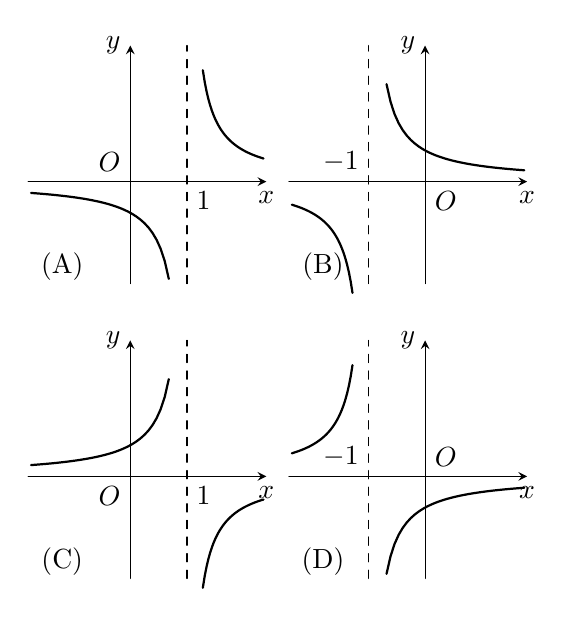
\begin{tikzpicture}[>=stealth,scale=0.72,line cap=round]
  % (A) 垂直渐近线 x = 1，双曲线递减分支
  \begin{scope}
    \draw[->] (-1.8,0)--(2.4,0) node[below] {$x$};
    \draw[->] (0,-1.8)--(0,2.4) node[left] {$y$};
    \node[above left] at (0,0) {$O$};
    \draw[dashed] (1,-1.8)--(1,2.4);
    \node[below right] at (1,0) {$1$};
    \draw[thick,domain=1.28:2.35,samples=35] plot (\x,{0.55/(\x-1)});
    \draw[thick,domain=-1.75:0.68,samples=35] plot (\x,{0.55/(\x-1)});
    \node at (-1.2,-1.5) {(A)};
  \end{scope}

  % (B) 垂直渐近线 x = -1，双曲线递减分支（正确选项）
  \begin{scope}[xshift=5.2cm]
    \draw[->] (-2.4,0)--(1.8,0) node[below] {$x$};
    \draw[->] (0,-1.8)--(0,2.4) node[left] {$y$};
    \node[below right] at (0,0) {$O$};
    \draw[dashed] (-1,-1.8)--(-1,2.4);
    \node[above left] at (-1,0) {$-1$};
    \draw[thick,domain=-0.68:1.75,samples=35] plot (\x,{0.55/(\x+1)});
    \draw[thick,domain=-2.35:-1.28,samples=35] plot (\x,{0.55/(\x+1)});
    \node at (-1.8,-1.5) {(B)};
  \end{scope}

  % (C) 垂直渐近线 x = 1，双曲线递增分支
  \begin{scope}[yshift=-5.2cm]
    \draw[->] (-1.8,0)--(2.4,0) node[below] {$x$};
    \draw[->] (0,-1.8)--(0,2.4) node[left] {$y$};
    \node[below left] at (0,0) {$O$};
    \draw[dashed] (1,-1.8)--(1,2.4);
    \node[below right] at (1,0) {$1$};
    \draw[thick,domain=1.28:2.35,samples=35] plot (\x,{-0.55/(\x-1)});
    \draw[thick,domain=-1.75:0.68,samples=35] plot (\x,{-0.55/(\x-1)});
    \node at (-1.2,-1.5) {(C)};
  \end{scope}

  % (D) 垂直渐近线 x = -1，双曲线递增分支
  \begin{scope}[xshift=5.2cm,yshift=-5.2cm]
    \draw[->] (-2.4,0)--(1.8,0) node[below] {$x$};
    \draw[->] (0,-1.8)--(0,2.4) node[left] {$y$};
    \node[above right] at (0,0) {$O$};
    \draw[dashed] (-1,-1.8)--(-1,2.4);
    \node[above left] at (-1,0) {$-1$};
    \draw[thick,domain=-0.68:1.75,samples=35] plot (\x,{-0.55/(\x+1)});
    \draw[thick,domain=-2.35:-1.28,samples=35] plot (\x,{-0.55/(\x+1)});
    \node at (-1.8,-1.5) {(D)};
  \end{scope}
\end{tikzpicture}\end{center}
\nopagebreak[4]
\Needspace{4\baselineskip}
\textbf{解析}

\Needspace{5\baselineskip}
原函数为 $y = \dfrac{1-x}{x}\ (x \neq 0)$，将其分离常数可得：
\nopagebreak[4]
\[
y = \dfrac{1}{x} - 1.
\]
\Needspace{5\baselineskip}
变形解出自变量 $x$：
\nopagebreak[4]
\[
y + 1 = \dfrac{1}{x} \iff x = \dfrac{1}{y + 1}.
\]
\Needspace{5\baselineskip}
互换 $x, y$，得到反函数解析式：
\nopagebreak[4]
\[
y = \dfrac{1}{x + 1} \quad (x \neq -1).
\]
分析该反函数的图象特征：
1. 渐近线：垂直渐近线为直线 $x = -1$，水平渐近线为 $x$ 轴（即直线 $y = 0$）；
2. 象限分支与单调性：由 $y = \dfrac{1}{x}$ 向左平移 $1$ 个单位得到，双曲线的两支位于由渐近线划分的右上方与左下方；
3. 特殊点：当 $x = 0$ 时，$y = 1$，图象过点 $(0, 1)$；当 $x > -1$ 时，$y > 0$，单调递减；当 $x < -1$ 时，$y < 0$，单调递减．

对比各选项图象：
选项 (B) 的垂直渐近线为虚线 $x = -1$，且在区间 $(-1, +\infty)$ 与 $(-\infty, -1)$ 上均为单调递减分支，过点 $(0, 1)$，符合要求．

故选 B．

\gkanswer{答案：B}

\end{answer}
\begin{answer}
\gksolhead{4}{}

\textbf{题目}：

已知函数 $y = \sin\left(x - \dfrac{\pi}{12}\right)\cos\left(x - \dfrac{\pi}{12}\right)$，则下列判断正确的是\mbox{（　　）}

\begin{gkopts}(1)
\task A．此函数的最小正周期为 $2\pi$，其图象的一个对称中心是 $\left(\dfrac{\pi}{12}, 0\right)$
\task B．此函数的最小正周期为 $\pi$，其图象的一个对称中心是 $\left(\dfrac{\pi}{12}, 0\right)$
\task C．此函数的最小正周期为 $2\pi$，其图象的一个对称中心是 $\left(\dfrac{\pi}{6}, 0\right)$
\task D．此函数的最小正周期为 $\pi$，其图象的一个对称中心是 $\left(\dfrac{\pi}{6}, 0\right)$
\end{gkopts}

\Needspace{4\baselineskip}
\textbf{解析}

\Needspace{5\baselineskip}
利用二倍角公式化简函数解析式：
\nopagebreak[4]
\[
y = \sin\left(x - \dfrac{\pi}{12}\right)\cos\left(x - \dfrac{\pi}{12}\right) = \dfrac{1}{2}\sin\left[2\left(x - \dfrac{\pi}{12}\right)\right] = \dfrac{1}{2}\sin\left(2x - \dfrac{\pi}{6}\right).
\]
\Needspace{5\baselineskip}
1. 最小正周期：
\nopagebreak[4]
\[
T = \dfrac{2\pi}{2} = \pi.
\]
\Needspace{5\baselineskip}
2. 对称中心：令正弦部分为零，即
\nopagebreak[4]
\[
2x - \dfrac{\pi}{6} = k\pi \quad (k \in \mathbf{Z}) \iff 2x = k\pi + \dfrac{\pi}{6} \iff x = \dfrac{k\pi}{2} + \dfrac{\pi}{12} \quad (k \in \mathbf{Z}).
\]
取 $k = 0$，得 $x = \dfrac{\pi}{12}$，此时函数值为 $0$，故 $\left(\dfrac{\pi}{12}, 0\right)$ 是图象的一个对称中心．

综上，函数的最小正周期为 $\pi$，对称中心为 $\left(\dfrac{\pi}{12}, 0\right)$．

故选 B．

\gkanswer{答案：B}

\end{answer}
\begin{answer}
\gksolhead{5}{}

\textbf{题目}：

下列函数既是奇函数，又在区间 $[-1, 1]$ 上单调递减的是\mbox{（　　）}

\begin{gkopts}(2)
\task A．$f(x) = \sin x$
\task B．$f(x) = -|x + 1|$
\task C．$f(x) = \dfrac{1}{2}(a^x + a^{-x})$
\task D．$f(x) = \ln \dfrac{2-x}{2+x}$
\end{gkopts}

\Needspace{4\baselineskip}
\textbf{解析}

逐一分析各选项：
\begin{itemize}
\item 选项 A：$f(x) = \sin x$ 是奇函数，但在区间 $[-1, 1] \subset \left[-\dfrac{\pi}{2}, \dfrac{\pi}{2}\right]$ 上单调递增，不符合题意；
\item 选项 B：$f(x) = -|x + 1|$，由于 $f(1) = -2$，$f(-1) = 0$，显然 $f(-1) \neq -f(1)$，非奇非偶函数，不符合题意；
\item 选项 C：$f(x) = \dfrac{1}{2}(a^x + a^{-x})$，满足 $f(-x) = f(x)$，为偶函数，不符合题意；
\item 选项 D：$f(x) = \ln \dfrac{2-x}{2+x}$：
\end{itemize}
  1. 定义域：由 $\dfrac{2-x}{2+x} > 0 \iff (2-x)(2+x) > 0$ 得定义域为 $(-2, 2)$，关于原点对称；
\Needspace{5\baselineskip}
  2. 奇偶性：
\nopagebreak[4]
\[
f(-x) = \ln \dfrac{2 - (-x)}{2 + (-x)} = \ln \dfrac{2+x}{2-x} = \ln \left(\dfrac{2-x}{2+x}\right)^{-1} = -\ln \dfrac{2-x}{2+x} = -f(x),
\]
  故 $f(x)$ 为奇函数；
  3. 单调性：内层函数 $g(x) = \dfrac{2-x}{2+x} = \dfrac{4-(2+x)}{2+x} = \dfrac{4}{x+2} - 1$．在区间 $[-1, 1]$ 上，$x+2$ 单调递增，故 $\dfrac{4}{x+2}-1$ 单调递减；外层对数函数 $y = \ln u$ 单调递增，由复合函数同增异减原则可知，$f(x)$ 在 $[-1, 1]$ 上单调递减．

故选 D．

\gkanswer{答案：D}

\end{answer}
\begin{answer}
\gksolhead{6}{}

\textbf{题目}：

如果 $\left(3x - \dfrac{1}{\sqrt[3]{x^2}}\right)^n$ 的展开式中各项系数之和为 $128$，则展开式中 $\dfrac{1}{x^3}$ 的系数是\mbox{（　　）}

\begin{gkopts}(4)
\task A．$7$
\task B．$-7$
\task C．$21$
\task D．$-21$
\end{gkopts}

\Needspace{4\baselineskip}
\textbf{解析}

1. 求展开式各项系数之和：
\Needspace{5\baselineskip}
在二项式 $\left(3x - \dfrac{1}{\sqrt[3]{x^2}}\right)^n$ 中，令 $x = 1$，各项系数之和为：
\nopagebreak[4]
\[
(3 - 1)^n = 2^n = 128 \implies n = 7.
\]
2. 求 $\dfrac{1}{x^3}$ 项的系数：
\Needspace{5\baselineskip}
展开式的通项公式为：
\nopagebreak[4]
\[
T_{r+1} = \mathrm{C}_7^r (3x)^{7-r} \left(-x^{-2/3}\right)^r = \mathrm{C}_7^r \cdot 3^{7-r} \cdot (-1)^r \cdot x^{7 - r - \frac{2}{3}r} = \mathrm{C}_7^r \cdot 3^{7-r} \cdot (-1)^r \cdot x^{7 - \frac{5}{3}r}.
\]
\Needspace{5\baselineskip}
令指数等于 $-3$：
\nopagebreak[4]
\[
7 - \dfrac{5}{3}r = -3 \iff \dfrac{5}{3}r = 10 \iff r = 6.
\]
\Needspace{5\baselineskip}
将 $r = 6$ 代入通项公式，系数为：
\nopagebreak[4]
\[
\mathrm{C}_7^6 \cdot 3^{7-6} \cdot (-1)^6 = 7 \cdot 3 \cdot 1 = 21.
\]

故选 C．

\gkanswer{答案：C}

\end{answer}
\begin{answer}
\gksolhead{7}{}

\textbf{题目}：

函数 $f(x) = \begin{cases} \sin(\pi x^2), & -1 < x < 0, \\ \mathrm{e}^{x-1}, & x \geqslant 0. \end{cases}$ 若 $f(1) + f(a) = 2$，则 $a$ 的所有可能值为\mbox{（　　）}

\begin{gkopts}(2)
\task A．$1$
\task B．$-\dfrac{\sqrt{2}}{2}$
\task C．$1, -\dfrac{\sqrt{2}}{2}$
\task D．$1, \dfrac{\sqrt{2}}{2}$
\end{gkopts}

\Needspace{4\baselineskip}
\textbf{解析}

由分段函数定义：
当 $x = 1 \geqslant 0$ 时，$f(1) = \mathrm{e}^{1-1} = \mathrm{e}^0 = 1$．
\Needspace{5\baselineskip}
已知 $f(1) + f(a) = 2$，故：
\nopagebreak[4]
\[
1 + f(a) = 2 \implies f(a) = 1.
\]
对实数 $a$ 分类讨论：
\Needspace{5\baselineskip}
1. 若 $a \geqslant 0$：
\nopagebreak[4]
\[
f(a) = \mathrm{e}^{a-1} = 1 \implies a - 1 = 0 \implies a = 1.
\]
满足 $a \geqslant 0$．
\Needspace{5\baselineskip}
2. 若 $-1 < a < 0$：
\nopagebreak[4]
\[
f(a) = \sin(\pi a^2) = 1.
\]
因为 $-1 < a < 0$，所以 $0 < a^2 < 1$，从而 $0 < \pi a^2 < \pi$．
\Needspace{5\baselineskip}
在区间 $(0, \pi)$ 内，满足正弦值为 $1$ 的角只有 $\dfrac{\pi}{2}$，即：
\nopagebreak[4]
\[
\pi a^2 = \dfrac{\pi}{2} \implies a^2 = \dfrac{1}{2} \implies a = -\dfrac{\sqrt{2}}{2} \quad (\text{\text{舍去正根，因为} } a < 0).
\]
满足 $-1 < a < 0$．

综上，$a$ 的所有可能值为 $1$ 或 $-\dfrac{\sqrt{2}}{2}$．

故选 C．

\gkanswer{答案：C}

\end{answer}
\begin{answer}
\gksolhead{8}{}

\textbf{题目}：

已知向量 $\vec{a}, \vec{b}$，且 $\vec{AB} = \vec{a} + 2\vec{b}$，$\vec{BC} = -5\vec{a} + 6\vec{b}$，$\vec{CD} = 7\vec{a} - 2\vec{b}$，则一定共线的三点是\mbox{（　　）}

\begin{gkopts}(2)
\task A．$A$、$B$、$D$
\task B．$A$、$B$、$C$
\task C．$B$、$C$、$D$
\task D．$A$、$C$、$D$
\end{gkopts}

\Needspace{4\baselineskip}
\textbf{解析}

计算各向量的线性组合：
\Needspace{5\baselineskip}
由题意，
\nopagebreak[4]
\[
\vec{AD} = \vec{AB} + \vec{BC} + \vec{CD} = (\vec{a} + 2\vec{b}) + (-5\vec{a} + 6\vec{b}) + (7\vec{a} - 2\vec{b}) = 3\vec{a} + 6\vec{b}.
\]
\Needspace{5\baselineskip}
注意到：
\nopagebreak[4]
\[
\vec{AB} = \vec{a} + 2\vec{b},
\]
\Needspace{5\baselineskip}
因此：
\nopagebreak[4]
\[
\vec{AD} = 3(\vec{a} + 2\vec{b}) = 3\vec{AB}.
\]
这表明向量 $\vec{AD}$ 与 $\vec{AB}$ 共线，且有公共点 $A$，因此 $A, B, D$ 三点一定共线．

故选 A．

\gkanswer{答案：A}

\end{answer}
\begin{answer}
\gksolhead{9}{}

\textbf{题目}：

设地球的半径为 $R$，若甲地位于北纬 $45^\circ$ 东经 $120^\circ$，乙地位于南纬 $75^\circ$ 东经 $120^\circ$，则甲、乙两地的球面距离为\mbox{（　　）}

\begin{gkopts}(2)
\task A．$\sqrt{3}R$
\task B．$\dfrac{\pi}{6}R$
\task C．$\dfrac{5\pi}{6}R$
\task D．$\dfrac{2\pi}{3}R$
\end{gkopts}

\Needspace{4\baselineskip}
\textbf{解析}

甲地位于北纬 $45^\circ$ 东经 $120^\circ$，乙地位于南纬 $75^\circ$ 东经 $120^\circ$．
\Needspace{5\baselineskip}
甲、乙两地位于同一条经线圈上，它们相对于地心的纬度跨度为：
\nopagebreak[4]
\[
\theta = 45^\circ + 75^\circ = 120^\circ.
\]
\Needspace{5\baselineskip}
将圆心角化为弧度制：
\nopagebreak[4]
\[
\theta = 120^\circ \times \dfrac{\pi}{180^\circ} = \dfrac{2\pi}{3}.
\]
\Needspace{5\baselineskip}
因此甲、乙两地的球面距离等于该大圆劣弧的长：
\nopagebreak[4]
\[
d = R \cdot \theta = \dfrac{2\pi}{3}R.
\]

故选 D．

\gkanswer{答案：D}

\end{answer}
\begin{answer}
\gksolhead{10}{}

\textbf{题目}：

$10$ 张奖券中只有 $3$ 张有奖，$5$ 个人购买，每人 $1$ 张，至少有 $1$ 人中奖的概率是\mbox{（　　）}

\begin{gkopts}(4)
\task A．$\dfrac{3}{10}$
\task B．$\dfrac{1}{12}$
\task C．$\dfrac{1}{2}$
\task D．$\dfrac{11}{12}$
\end{gkopts}

\Needspace{4\baselineskip}
\textbf{解析}

设有 $10$ 张奖券，其中有奖的 $3$ 张，无奖的 $7$ 张．
$5$ 个人购买，每人 $1$ 张，样本空间中从 $10$ 张中任取 $5$ 张的样本点总数为 $\mathrm{C}_{10}^5$．
考虑所求事件“至少有 $1$ 人中奖”的对立事件：“$5$ 人均未中奖”，即取出的 $5$ 张奖券均来自无奖的 $7$ 张奖券．
\Needspace{5\baselineskip}
对立事件的概率为：
\nopagebreak[4]
\[
P(\text{\text{均未中奖}}) = \dfrac{\mathrm{C}_7^5}{\mathrm{C}_{10}^5} = \dfrac{\mathrm{C}_7^2}{\mathrm{C}_{10}^5} = \dfrac{\dfrac{7 \times 6}{2}}{\dfrac{10 \times 9 \times 8 \times 7 \times 6}{5 \times 4 \times 3 \times 2 \times 1}} = \dfrac{21}{252} = \dfrac{1}{12}.
\]
\Needspace{5\baselineskip}
因此至少有 $1$ 人中奖的概率为：
\nopagebreak[4]
\[
P = 1 - P(\text{\text{均未中奖}}) = 1 - \dfrac{1}{12} = \dfrac{11}{12}.
\]

故选 D．

\gkanswer{答案：D}

\end{answer}
\begin{answer}
\gksolhead{11}{}

\textbf{题目}：

设集合 $A$、$B$ 是全集 $U$ 的两个子集，则 $A \subsetneqq B$ 是 $(\complement_U A) \cup B = U$ 的\mbox{（　　）}

\begin{gkopts}(2)
\task A．充分不必要条件
\task B．必要不充分条件
\task C．充要条件
\task D．既不充分也不必要条件
\end{gkopts}

\Needspace{4\baselineskip}
\textbf{解析}

首先分析命题 $(\complement_U A) \cup B = U$ 的充要条件：
\begin{itemize}
\item 若 $A \subseteq B$，对于全集 $U$ 中的任一元素 $x$：若 $x \in A$，则必有 $x \in B$；若 $x \notin A$，则 $x \in \complement_U A$．故总有 $x \in (\complement_U A) \cup B$，因此 $(\complement_U A) \cup B = U$；
\item 反之，若 $(\complement_U A) \cup B = U$，假设存在 $x \in A$ 且 $x \notin B$，则 $x \notin \complement_U A$ 且 $x \notin B$，从而 $x \notin (\complement_U A) \cup B$，与并集为 $U$ 矛盾．故必有 $A \subseteq B$．
\end{itemize}
因此，$(\complement_U A) \cup B = U \iff A \subseteq B$．

现在考察条件 $A \subsetneqq B$：
\begin{itemize}
\item 充分性：若 $A \subsetneqq B$，则显然有 $A \subseteq B$，故 $(\complement_U A) \cup B = U$ 成立，充分性具备；
\item 必要性：若 $(\complement_U A) \cup B = U$，即 $A \subseteq B$，此时可能存在 $A = B$，不一定满足真包含关系 $A \subsetneqq B$，必要性不具备．
\end{itemize}

综上，$A \subsetneqq B$ 是 $(\complement_U A) \cup B = U$ 的充分不必要条件．

故选 A．

\gkanswer{答案：A}

\end{answer}
\begin{answer}
\gksolhead{12}{}

\textbf{题目}：

设直线 $l: 2x + y + 2 = 0$ 关于原点对称的直线为 $l'$，若 $l'$ 与椭圆 $x^2 + \dfrac{y^2}{4} = 1$ 的交点为 $A$、$B$，点 $P$ 为椭圆上的动点，则使 $\triangle PAB$ 的面积为 $\dfrac{1}{2}$ 的点 $P$ 的个数为\mbox{（　　）}

\begin{gkopts}(4)
\task A．$1$
\task B．$2$
\task C．$3$
\task D．$4$
\end{gkopts}

\Needspace{4\baselineskip}
\textbf{解析}

1. 求对称直线 $l'$ 的方程：
\Needspace{5\baselineskip}
直线 $l: 2x + y + 2 = 0$ 关于原点对称，只需将 $(x, y)$ 替换为 $(-x, -y)$：
\nopagebreak[4]
\[
2(-x) + (-y) + 2 = 0 \iff -2x - y + 2 = 0 \iff 2x + y - 2 = 0.
\]
故直线 $l'$ 的方程为 $2x + y - 2 = 0$．
2. 求直线 $l'$ 与椭圆的交点及弦长：
\Needspace{5\baselineskip}
联立直线 $l'$ 与椭圆方程：
\nopagebreak[4]
\[
\begin{cases} 2x + y - 2 = 0 \implies y = 2 - 2x, \\ x^2 + \dfrac{y^2}{4} = 1. \end{cases}
\]
\Needspace{5\baselineskip}
代入得：
\nopagebreak[4]
\[
x^2 + \dfrac{(2-2x)^2}{4} = 1 \iff x^2 + (1-x)^2 = 1 \iff 2x^2 - 2x = 0 \iff 2x(x - 1) = 0.
\]
解得 $x_1 = 0 \implies y_1 = 2$，$x_2 = 1 \implies y_2 = 0$．
两交点坐标为 $A(0, 2)$，$B(1, 0)$．
\Needspace{5\baselineskip}
弦长为：
\nopagebreak[4]
\[
|AB| = \sqrt{(1 - 0)^2 + (0 - 2)^2} = \sqrt{1 + 4} = \sqrt{5}.
\]
3. 求三角形面积条件：
设椭圆上的动点 $P$ 到直线 $l'$ 的距离为 $d$．
\Needspace{5\baselineskip}
三角形面积为：
\nopagebreak[4]
\[
S_{\triangle PAB} = \dfrac{1}{2} |AB| \cdot d = \dfrac{\sqrt{5}}{2} d.
\]
\Needspace{5\baselineskip}
依题意，$S_{\triangle PAB} = \dfrac{1}{2}$，从而：
\nopagebreak[4]
\[
\dfrac{\sqrt{5}}{2} d = \dfrac{1}{2} \implies d = \dfrac{1}{\sqrt{5}}.
\]
4. 判定满足距离条件的动点个数：
设与直线 $l': 2x + y - 2 = 0$ 平行且距离为 $\dfrac{1}{\sqrt{5}}$ 的直线为 $L: 2x + y + c = 0$．
\Needspace{5\baselineskip}
由两平行线间距离公式：
\nopagebreak[4]
\[
\dfrac{|c - (-2)|}{\sqrt{2^2 + 1^2}} = \dfrac{|c + 2|}{\sqrt{5}} = \dfrac{1}{\sqrt{5}} \implies |c + 2| = 1 \implies c = -1 \text{ \text{或} } c = -3.
\]
\Needspace{5\baselineskip}
即对应的两条直线为：
\nopagebreak[4]
\[
L_1: 2x + y - 1 = 0, \quad L_2: 2x + y - 3 = 0.
\]
考察与椭圆平行的切线截距：
\Needspace{5\baselineskip}
设椭圆的切线为 $2x + y + m = 0 \implies y = -2x - m$．代入椭圆方程得：
\nopagebreak[4]
\[
x^2 + \dfrac{(-2x-m)^2}{4} = 1 \implies 8x^2 + 4mx + m^2 - 4 = 0.
\]
\Needspace{5\baselineskip}
判别式：
\nopagebreak[4]
\[
\Delta = 16m^2 - 32(m^2 - 4) = 16(8 - m^2) = 0 \implies m = \pm 2\sqrt{2}.
\]
切线的常数项范围为 $[-2\sqrt{2}, 2\sqrt{2}]$，由于 $2\sqrt{2} = \sqrt{8} \approx 2.828$：
\begin{itemize}
\item 对于直线 $L_1: 2x + y - 1 = 0$，其常数项 $-1 \in (-2\sqrt{2}, 2\sqrt{2})$，因此直线 $L_1$ 与椭圆相交于 $2$ 个不同点；
\item 对于直线 $L_2: 2x + y - 3 = 0$，其常数项 $-3 < -2\sqrt{2}$（即 $2x+y=3 > 2\sqrt{2}$），直线 $L_2$ 与椭圆相离，无公共点．
\end{itemize}
因此，椭圆上满足 $\triangle PAB$ 面积为 $\dfrac{1}{2}$ 的点 $P$ 恰有 $2$ 个．

故选 B．

\gkanswer{答案：B}

\end{answer}
\begin{answer}
\gksolhead{13}{}

\textbf{题目}：

某学校共有教师 $490$ 人，其中不到 $40$ 岁的有 $350$ 人，$40$ 岁及以上的有 $140$ 人，为了解普通话在该校教师中的推广普及情况，用分层抽样的方法，从全体教师中抽取一个容量为 $70$ 人的样本进行普通话水平测试，其中在不到 $40$ 岁的教师中应抽取的人数是 $\underline{\hspace{2em}}$．

\Needspace{4\baselineskip}
\textbf{解析}

全校教师共有 $490$ 人，其中不到 $40$ 岁的教师有 $350$ 人．
\Needspace{5\baselineskip}
不到 $40$ 岁的教师占全体教师的比例为：
\nopagebreak[4]
\[
\dfrac{350}{490} = \dfrac{5}{7}.
\]
\Needspace{5\baselineskip}
采用分层抽样抽取样本容量为 $70$ 人的样本，在不到 $40$ 岁的教师中应抽取的人数为：
\nopagebreak[4]
\[
70 \times \dfrac{5}{7} = 50.
\]

故答案为 $50$．

\gkanswer{答案：$50$。}

\end{answer}
\begin{answer}
\gksolhead{14}{}

\textbf{题目}：

设双曲线 $\dfrac{x^2}{a^2} - \dfrac{y^2}{b^2} = 1\ (a > 0, b > 0)$ 的右焦点为 $F$，右准线 $l$ 与两条渐近线交于 $P$、$Q$ 两点，如果 $\triangle PQF$ 是直角三角形，则双曲线的离心率 $e = \underline{\hspace{2em}}$．

\Needspace{4\baselineskip}
\textbf{解析}

双曲线方程为 $\dfrac{x^2}{a^2} - \dfrac{y^2}{b^2} = 1\ (a > 0, b > 0)$，其右焦点为 $F(c, 0)$，右准线方程为 $l: x = \dfrac{a^2}{c}$．
双曲线的两条渐近线方程为 $y = \pm \dfrac{b}{a} x$．
\Needspace{5\baselineskip}
准线 $l$ 与两条渐近线的交点为：
\nopagebreak[4]
\[
P\left(\dfrac{a^2}{c}, \dfrac{ab}{c}\right), \quad Q\left(\dfrac{a^2}{c}, -\dfrac{ab}{c}\right).
\]
线段 $PQ$ 垂直于 $x$ 轴，对称轴为 $x$ 轴，且中点为 $H\left(\dfrac{a^2}{c}, 0\right)$．
因为 $F(c, 0)$ 在对称轴 $x$ 轴上，所以 $|FP| = |FQ|$，$\triangle PQF$ 是以 $F$ 为顶点的等腰三角形．
已知 $\triangle PQF$ 是直角三角形，故直角必为 $\angle PFQ = 90^\circ$．
\Needspace{5\baselineskip}
在等腰直角三角形中，$FH \perp PQ$ 且平分 $\angle PFQ$，因此 $\angle PFH = 45^\circ$，从而有：
\nopagebreak[4]
\[
|PH| = |HF|.
\]
\Needspace{5\baselineskip}
计算线段长度：
\nopagebreak[4]
\[
|PH| = \dfrac{ab}{c}, \quad |HF| = c - \dfrac{a^2}{c} = \dfrac{c^2 - a^2}{c} = \dfrac{b^2}{c}.
\]
\Needspace{5\baselineskip}
代入得：
\nopagebreak[4]
\[
\dfrac{ab}{c} = \dfrac{b^2}{c} \implies a = b.
\]
\Needspace{5\baselineskip}
此时双曲线为等轴双曲线，其离心率为：
\nopagebreak[4]
\[
e = \dfrac{c}{a} = \sqrt{1 + \dfrac{b^2}{a^2}} = \sqrt{1 + 1} = \sqrt{2}.
\]

故答案为 $\sqrt{2}$．

\gkanswer{答案：$\sqrt{2}$。}

\end{answer}
\begin{answer}
\gksolhead{15}{}

\textbf{题目}：

设 $x, y$ 满足约束条件 $\begin{cases} x + y \leqslant 5, \\ 3x + 2y \leqslant 12, \\ 0 \leqslant x \leqslant 3, \\ 0 \leqslant y \leqslant 4, \end{cases}$ 则使得目标函数 $z = 6x + 5y$ 最大的点 $(x, y)$ 是 $\underline{\hspace{2em}}$．

\Needspace{4\baselineskip}
\textbf{解析}

\Needspace{5\baselineskip}
约束条件为：
\nopagebreak[4]
\[
\begin{cases}
x + y \leqslant 5, \\
3x + 2y \leqslant 12, \\
0 \leqslant x \leqslant 3, \\
0 \leqslant y \leqslant 4.
\end{cases}
\]
画出可行域，其顶点坐标分析如下：
1. 联立 $x + y = 5$ 与 $3x + 2y = 12$：
由第一式 $y = 5 - x$，代入第二式得 $3x + 2(5 - x) = 12 \implies x = 2, y = 3$．
验证满足 $0 \leqslant x \leqslant 3, 0 \leqslant y \leqslant 4$，交点为 $(2, 3)$．
2. 联立 $3x + 2y = 12$ 与 $x = 3$：解得 $y = 1.5$．交点为 $(3, 1.5)$；
3. 联立 $x + y = 5$ 与 $y = 4$：解得 $x = 1$．交点为 $(1, 4)$；
4. 其它边界交点：$(3, 0), (0, 0), (0, 4)$．

将各顶点代入目标函数 $z = 6x + 5y$：
\begin{itemize}
\item 代入 $(2, 3)$：$z = 6(2) + 5(3) = 12 + 15 = 27$；
\item 代入 $(3, 1.5)$：$z = 6(3) + 5(1.5) = 18 + 7.5 = 25.5$；
\item 代入 $(1, 4)$：$z = 6(1) + 5(4) = 6 + 20 = 26$；
\item 代入 $(3, 0)$：$z = 18$；
\item 代入 $(0, 4)$：$z = 20$；
\item 代入 $(0, 0)$：$z = 0$．
\end{itemize}

比较可知，$z$ 的最大值为 $27$，此时对应的点 $(x, y)$ 为 $(2, 3)$．

故答案为 $(2, 3)$．

\gkanswer{答案：$(2, 3)$。}

\end{answer}
\begin{answer}
\gksolhead{16}{}

\textbf{题目}：

已知 $m, n$ 是不同的直线，$\alpha, \beta$ 是不重合的平面，给出下列命题：
① 若 $m \parallel \alpha$，则 $m$ 平行于平面 $\alpha$ 内的任一条直线；
② 若 $\alpha \parallel \beta$，$m \subset \alpha$，$n \subset \beta$，则 $m \parallel n$；
③ 若 $m \perp \alpha$，$n \perp \beta$，$m \parallel n$，则 $\alpha \parallel \beta$；
④ 若 $\alpha \parallel \beta$，$m \subset \alpha$，则 $m \parallel \beta$．
上面的命题中，真命题的序号是 $\underline{\hspace{2em}}$．（写出所有真命题的序号）

\Needspace{4\baselineskip}
\textbf{解析}

逐一分析各命题：
\begin{itemize}
\item ① 若 $m \parallel \alpha$，则直线 $m$ 平行于平面 $\alpha$，但在平面 $\alpha$ 内除了与 $m$ 平行的直线外，其余与 $m$ 不平行的直线均与 $m$ 异面，故①为假命题；
\item ② 若 $\alpha \parallel \beta$，$m \subset \alpha$，$n \subset \beta$，两平面平行，平面内的两条直线无公共点，它们可以平行，也可以异面，故②为假命题；
\item ③ 若 $m \perp \alpha$，$n \perp \beta$，则直线 $m, n$ 分别为两平面的法向量所在直线．又 $m \parallel n$，说明两平面的法向量平行，且两平面不重合，故 $\alpha \parallel \beta$ 成立，③为真命题；
\item ④ 若 $\alpha \parallel \beta$，$m \subset \alpha$，两平面平行则没有公共点，直线 $m$ 在平面 $\alpha$ 内，因而直线 $m$ 与平面 $\beta$ 也无公共点，由线面平行的定义可知 $m \parallel \beta$ 成立，④为真命题．
\end{itemize}

上面的命题中，真命题的序号是 ③④．

故答案为 ③④．

\gkanswer{答案：③④。}

\end{answer}
\begin{answer}
\gksolhead{17}{}

\textbf{题目}：

已知向量 $\vec{m} = (\cos\theta, \sin\theta)$ 和 $\vec{n} = (\sqrt{2}-\sin\theta, \cos\theta)$，$\theta \in (\pi, 2\pi)$，且 $|\vec{m} + \vec{n}| = \dfrac{8\sqrt{2}}{5}$，求 $\cos\left(\dfrac{\theta}{2} + \dfrac{\pi}{8}\right)$ 的值．

\Needspace{4\baselineskip}
\textbf{解析}

由题意，向量 $\vec{m} = (\cos\theta, \sin\theta)$，$\vec{n} = (\sqrt{2}-\sin\theta, \cos\theta)$．
\Needspace{5\baselineskip}
计算和向量：
\nopagebreak[4]
\[
\vec{m} + \vec{n} = (\cos\theta - \sin\theta + \sqrt{2}, \sin\theta + \cos\theta).
\]
\Needspace{5\baselineskip}
其模长的平方为：
\nopagebreak[4]
\[
|\vec{m} + \vec{n}|^2 = (\cos\theta - \sin\theta + \sqrt{2})^2 + (\sin\theta + \cos\theta)^2.
\]
\Needspace{5\baselineskip}
展开第一项：
\nopagebreak[4]
\[
(\cos\theta - \sin\theta + \sqrt{2})^2 = (\cos\theta - \sin\theta)^2 + 2\sqrt{2}(\cos\theta - \sin\theta) + 2.
\]
\Needspace{5\baselineskip}
结合第二项，注意到：
\nopagebreak[4]
\[
(\cos\theta - \sin\theta)^2 + (\sin\theta + \cos\theta)^2 = 2(\cos^2\theta + \sin^2\theta) = 2.
\]
\Needspace{5\baselineskip}
因此：
\nopagebreak[4]
\[
|\vec{m} + \vec{n}|^2 = 2 + 2\sqrt{2}(\cos\theta - \sin\theta) + 2 = 4 + 2\sqrt{2}(\cos\theta - \sin\theta).
\]
\Needspace{5\baselineskip}
已知 $|\vec{m} + \vec{n}| = \dfrac{8\sqrt{2}}{5}$，平方得：
\nopagebreak[4]
\[
|\vec{m} + \vec{n}|^2 = \left(\dfrac{8\sqrt{2}}{5}\right)^2 = \dfrac{128}{25}.
\]
\Needspace{5\baselineskip}
代入等式解出 $\cos\theta - \sin\theta$：
\nopagebreak[4]
\[
4 + 2\sqrt{2}(\cos\theta - \sin\theta) = \dfrac{128}{25} \implies 2\sqrt{2}(\cos\theta - \sin\theta) = \dfrac{28}{25} \implies \cos\theta - \sin\theta = \dfrac{7\sqrt{2}}{25}.
\]
\Needspace{5\baselineskip}
利用辅助角公式化简：
\nopagebreak[4]
\[
\cos\theta - \sin\theta = \sqrt{2}\left(\dfrac{\sqrt{2}}{2}\cos\theta - \dfrac{\sqrt{2}}{2}\sin\theta\right) = \sqrt{2}\cos\left(\theta + \dfrac{\pi}{4}\right).
\]
\Needspace{5\baselineskip}
从而：
\nopagebreak[4]
\[
\sqrt{2}\cos\left(\theta + \dfrac{\pi}{4}\right) = \dfrac{7\sqrt{2}}{25} \implies \cos\left(\theta + \dfrac{\pi}{4}\right) = \dfrac{7}{25}.
\]
\Needspace{5\baselineskip}
令 $\alpha = \dfrac{\theta}{2} + \dfrac{\pi}{8}$，则 $2\alpha = \theta + \dfrac{\pi}{4}$．由二倍角余弦公式：
\nopagebreak[4]
\[
\cos(2\alpha) = 2\cos^2\alpha - 1 \implies 2\cos^2\left(\dfrac{\theta}{2} + \dfrac{\pi}{8}\right) = 1 + \cos\left(\theta + \dfrac{\pi}{4}\right) = 1 + \dfrac{7}{25} = \dfrac{32}{25}.
\]
\Needspace{5\baselineskip}
解得：
\nopagebreak[4]
\[
\cos^2\left(\dfrac{\theta}{2} + \dfrac{\pi}{8}\right) = \dfrac{16}{25}.
\]
确定符号：
因为 $\theta \in (\pi, 2\pi)$，所以 $\dfrac{\theta}{2} \in \left(\dfrac{\pi}{2}, \pi\right)$，
\Needspace{5\baselineskip}
从而：
\nopagebreak[4]
\[
\dfrac{\theta}{2} + \dfrac{\pi}{8} \in \left(\dfrac{5\pi}{8}, \dfrac{9\pi}{8}\right).
\]
由于 $\dfrac{\pi}{2} < \dfrac{5\pi}{8} < \dfrac{9\pi}{8} < \dfrac{3\pi}{2}$，角 $\dfrac{\theta}{2} + \dfrac{\pi}{8}$ 位于第二或第三象限，其余弦值必为负数．
\Needspace{5\baselineskip}
故：
\nopagebreak[4]
\[
\cos\left(\dfrac{\theta}{2} + \dfrac{\pi}{8}\right) = -\dfrac{4}{5}.
\]

\gkanswer{答案：$-\dfrac{4}{5}$。}

\end{answer}
\begin{answer}
\gksolhead{18}{}

\textbf{题目}：

袋中装有黑球和白球共 $7$ 个，从中任取 $2$ 个球都是白球的概率为 $\dfrac{1}{7}$，现有甲、乙两人从袋中轮流摸取 $1$ 球，甲先取，乙后取，然后甲再取 $\cdots\cdots$，取后不放回，直到两人中有一人取到白球时既终止，每个球在每一次被取出的机会是等可能的．
(1) 求袋中原有的白球的个数；
(2) 求取球 $2$ 次终止的概率；
(3) 求甲取到白球的概率．

\Needspace{4\baselineskip}
\textbf{解析}

\textbf{(1)}
设袋中原有白球 $k$ 个（$k \in \{2, 3, 4, 5, 6, 7\}$），则黑球有 $7 - k$ 个．
\Needspace{5\baselineskip}
从袋中任取 $2$ 个球都是白球的概率为：
\nopagebreak[4]
\[
P = \dfrac{\mathrm{C}_k^2}{\mathrm{C}_7^2} = \dfrac{k(k-1)}{21} = \dfrac{1}{7}.
\]
\Needspace{5\baselineskip}
解得：
\nopagebreak[4]
\[
k(k-1) = 3 \implies k^2 - k - 6 = 0 \implies (k - 3)(k + 2) = 0.
\]
由于 $k > 0$，得 $k = 3$．
因此袋中原有白球 $3$ 个，黑球 $4$ 个．

\textbf{(2)}
取球 $2$ 次终止，意味着第 $1$ 次甲取到黑球，第 $2$ 次乙取到白球．
\Needspace{5\baselineskip}
其概率为：
\nopagebreak[4]
\[
P = \dfrac{4}{7} \times \dfrac{3}{6} = \dfrac{4}{7} \times \dfrac{1}{2} = \dfrac{2}{7}.
\]

\textbf{(3)}
甲取到白球即摸球在第 $1$ 次、第 $3$ 次或第 $5$ 次终止（黑球仅 $4$ 个，最迟第 $5$ 次终止）：
\begin{itemize}
\item 第 $1$ 次终止（甲直接取到白球）：
\end{itemize}
\nopagebreak[4]
\[
P_1 = \dfrac{3}{7};
\]
\begin{itemize}
\item 第 $3$ 次终止（甲摸黑、乙摸黑、甲摸白）：
\end{itemize}
\nopagebreak[4]
\[
P_3 = \dfrac{4}{7} \times \dfrac{3}{6} \times \dfrac{3}{5} = \dfrac{2}{7} \times \dfrac{3}{5} = \dfrac{6}{35};
\]
\begin{itemize}
\item 第 $5$ 次终止（甲黑、乙黑、甲黑、乙黑、甲白）：
\end{itemize}
\nopagebreak[4]
\[
P_5 = \dfrac{4}{7} \times \dfrac{3}{6} \times \dfrac{2}{5} \times \dfrac{1}{4} \times \dfrac{3}{3} = \dfrac{2}{7} \times \dfrac{1}{10} \times 1 = \dfrac{1}{35}.
\]
\Needspace{5\baselineskip}
因为这三种情况互斥，故甲取到白球的概率为：
\nopagebreak[4]
\[
P = P_1 + P_3 + P_5 = \dfrac{3}{7} + \dfrac{6}{35} + \dfrac{1}{35} = \dfrac{15 + 6 + 1}{35} = \dfrac{22}{35}.
\]

\gkanswer{答案（1）：袋中原有白球 $3$ 个。}

\gkanswer{答案（2）：取球 $2$ 次终止的概率为 $\dfrac{2}{7}$。}

\gkanswer{答案（3）：甲取到白球的概率为 $\dfrac{22}{35}$。}

\end{answer}
\begin{answer}
\gksolhead{19}{}

\textbf{题目}：

已知 $x = 1$ 是函数 $f(x) = mx^3 - 3(m+1)x^2 + nx + 1$ 的一个极值点，其中 $m, n \in \mathbf{R}$，$m < 0$．
(1) 求 $m$ 与 $n$ 的关系式；
(2) 求 $f(x)$ 的单调区间．

\Needspace{4\baselineskip}
\textbf{解析}

\Needspace{5\baselineskip}
函数 $f(x) = mx^3 - 3(m+1)x^2 + nx + 1$ 的导数为：
\nopagebreak[4]
\[
f'(x) = 3mx^2 - 6(m+1)x + n.
\]

\textbf{(1)}
\Needspace{5\baselineskip}
已知 $x = 1$ 是函数 $f(x)$ 的一个极值点，由极值点的必要条件知 $f'(1) = 0$：
\nopagebreak[4]
\[
f'(1) = 3m(1)^2 - 6(m+1)(1) + n = 3m - 6m - 6 + n = -3m - 6 + n = 0.
\]
\Needspace{5\baselineskip}
解得：
\nopagebreak[4]
\[
n = 3m + 6.
\]

\textbf{(2)}
\Needspace{5\baselineskip}
将 $n = 3m + 6$ 代入导数表达式：
\nopagebreak[4]
\[
f'(x) = 3mx^2 - 6(m+1)x + 3m + 6 = 3\left[mx^2 - 2(m+1)x + m + 2\right].
\]
\Needspace{5\baselineskip}
对中括号内的二次三项式因式分解：
\nopagebreak[4]
\[
mx^2 - 2(m+1)x + m + 2 = (x - 1)[mx - (m+2)].
\]
\Needspace{5\baselineskip}
令 $f'(x) = 0$，解得两个根：
\nopagebreak[4]
\[
x_1 = 1, \quad x_2 = \dfrac{m+2}{m} = 1 + \dfrac{2}{m}.
\]
\Needspace{5\baselineskip}
已知 $m < 0$，因此 $\dfrac{2}{m} < 0$，从而：
\nopagebreak[4]
\[
x_2 = 1 + \dfrac{2}{m} < 1 = x_1.
\]
又因为二次项系数 $3m < 0$，抛物线开口向下：
\begin{itemize}
\item 当 $x < 1 + \dfrac{2}{m}$ 时，$f'(x) < 0$；
\item 当 $1 + \dfrac{2}{m} < x < 1$ 时，$f'(x) > 0$；
\item 当 $x > 1$ 时，$f'(x) < 0$．
\end{itemize}

在 $x = 1$ 处导数由正变负，确实取得极大值，满足极值点条件．
因此，函数 $f(x)$ 的单调递增区间为 $\left(1 + \dfrac{2}{m}, 1\right)$；
单调递减区间为 $\left(-\infty, 1 + \dfrac{2}{m}\right)$ 和 $(1, +\infty)$．

\gkanswer{答案（1）：$n = 3m + 6$。}

\gkanswer{答案（2）：函数 $f(x)$ 的单调递增区间为 $\left(1 + \dfrac{2}{m}, 1\right)$；单调递减区间为 $\left(-\infty, 1 + \dfrac{2}{m}\right)$ 和 $(1, +\infty)$。}

\end{answer}
\begin{answer}
\gksolhead{20}{}

\textbf{题目}：

如图，已知长方体 $ABCD - A_1B_1C_1D_1$，$AB = 2$，$AA_1 = 1$，直线 $BD$ 与平面 $AA_1B_1B$ 所成的角为 $30^\circ$，$AE$ 垂直 $BD$ 于 $E$，$F$ 为 $A_1B_1$ 的中点．
(1) 求异面直线 $AE$ 与 $BF$ 所成的角；
(2) 求平面 $BDF$ 与平面 $AA_1B$ 所成的二面角（锐角）的大小；
(3) 求点 $A$ 到平面 $BDF$ 的距离．
\nopagebreak[4]
\begin{center}% 2005 年山东卷文科第 20 题：长方体直观图与辅助线
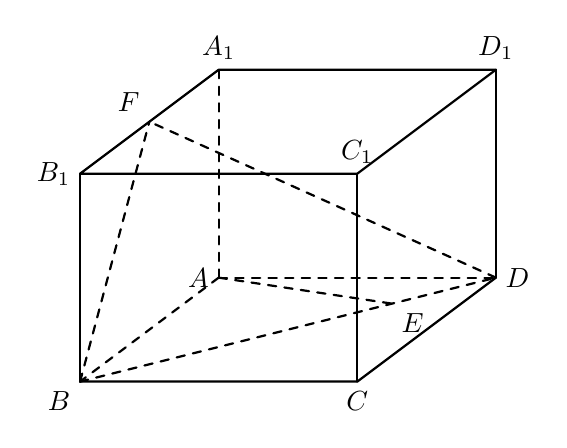
\begin{tikzpicture}[>=stealth,scale=1.1,line cap=round,line join=round]
  % 坐标定义
  % 底面顶点
  \coordinate (A) at (0,0);
  \coordinate (B) at (-1.6,-1.2);
  \coordinate (C) at (1.6,-1.2);
  \coordinate (D) at (3.2,0);

  % 顶面顶点（竖直高度 2.4）
  \coordinate (A1) at (0,2.4);
  \coordinate (B1) at (-1.6,1.2);
  \coordinate (C1) at (1.6,1.2);
  \coordinate (D1) at (3.2,2.4);

  % 中点与垂足
  \coordinate (F) at (-0.8,1.8); % A1B1 中点
  \coordinate (E) at (2.0,-0.3); % AE 垂直 BD 于 E (落在 CC1 右后方)

  % 虚线（不可见棱与辅助线）
  \draw[dashed,thick] (A) -- (A1);
  \draw[dashed,thick] (A) -- (B);
  \draw[dashed,thick] (A) -- (D);
  \draw[dashed,thick] (A) -- (E);
  \draw[dashed,thick] (B) -- (D);
  \draw[dashed,thick] (B) -- (F);
  \draw[dashed,thick] (D) -- (F);

  % 实线（可见棱）
  \draw[thick] (B) -- (C) -- (D);
  \draw[thick] (B) -- (B1);
  \draw[thick] (C) -- (C1);
  \draw[thick] (D) -- (D1);
  \draw[thick] (A1) -- (B1) -- (C1) -- (D1) -- cycle;

  % 顶点标签
  \node[above] at (A1) {$A_1$};
  \node[above] at (D1) {$D_1$};
  \node[left] at (B1) {$B_1$};
  \node[above] at (C1) {$C_1$};
  \node[above left] at (F) {$F$};
  \node[left] at (A) {$A$};
  \node[right] at (D) {$D$};
  \node[below left] at (B) {$B$};
  \node[below] at (C) {$C$};
  \node[below right] at (E) {$E$};
\end{tikzpicture}\end{center}
\nopagebreak[4]
\Needspace{4\baselineskip}
\textbf{解析}

在长方体 $ABCD - A_1B_1C_1D_1$ 中，因为 $DA \perp$ 平面 $AA_1B_1B$，所以 $BA$ 是直线 $BD$ 在平面 $AA_1B_1B$ 上的射影．
因此 $\angle DBA$ 为直线 $BD$ 与平面 $AA_1B_1B$ 所成的角，由已知得 $\angle DBA = 30^\circ$．
\Needspace{5\baselineskip}
在 Rt$\triangle DAB$ 中，$AB = 2$：
\nopagebreak[4]
\[
AD = AB \cdot \tan 30^\circ = 2 \times \dfrac{\sqrt{3}}{3} = \dfrac{2\sqrt{3}}{3}.
\]
以 $A$ 为原点，$AB$ 所在直线为 $x$ 轴，$AD$ 所在直线为 $y$ 轴，$AA_1$ 所在直线为 $z$ 轴建立空间直角坐标系：
\begin{itemize}
\item $A(0, 0, 0)$，$B(2, 0, 0)$，$D\left(0, \dfrac{2\sqrt{3}}{3}, 0\right)$，$C\left(2, \dfrac{2\sqrt{3}}{3}, 0\right)$；
\item $A_1(0, 0, 1)$，$B_1(2, 0, 1)$，$F$ 为 $A_1B_1$ 的中点，故 $F(1, 0, 1)$．
\end{itemize}

在底面矩形 $ABCD$ 中，$AE \perp BD$ 于 $E$．
直线 $BD$ 的截距方程为 $\dfrac{x}{2} + \dfrac{y}{2\sqrt{3}/3} = 1 \iff x + \sqrt{3}y - 2 = 0$．
过 $A(0, 0, 0)$ 且垂直于 $BD$ 的直线方程为 $\sqrt{3}x - y = 0 \iff y = \sqrt{3}x$．
联立得 $x + \sqrt{3}(\sqrt{3}x) - 2 = 0 \implies 4x = 2 \implies x = \dfrac{1}{2}$，$y = \dfrac{\sqrt{3}}{2}$．
故垂足 $E$ 的坐标为 $\left(\dfrac{1}{2}, \dfrac{\sqrt{3}}{2}, 0\right)$．

\textbf{(1)}
求异面直线 $AE$ 与 $BF$ 所成的角：
\Needspace{5\baselineskip}
向量 $\vec{AE} = \left(\dfrac{1}{2}, \dfrac{\sqrt{3}}{2}, 0\right)$，其模长为：
\nopagebreak[4]
\[
|\vec{AE}| = \sqrt{\left(\dfrac{1}{2}\right)^2 + \left(\dfrac{\sqrt{3}}{2}\right)^2 + 0} = 1.
\]
\Needspace{5\baselineskip}
向量 $\vec{BF} = F - B = (-1, 0, 1)$，其模长为：
\nopagebreak[4]
\[
|\vec{BF}| = \sqrt{(-1)^2 + 0^2 + 1^2} = \sqrt{2}.
\]
\Needspace{5\baselineskip}
计算内积：
\nopagebreak[4]
\[
\vec{AE} \cdot \vec{BF} = \dfrac{1}{2}(-1) + \dfrac{\sqrt{3}}{2}(0) + 0(1) = -\dfrac{1}{2}.
\]
\Needspace{5\baselineskip}
设异面直线 $AE$ 与 $BF$ 所成的角为 $\theta_1$，则：
\nopagebreak[4]
\[
\cos\theta_1 = \dfrac{|\vec{AE} \cdot \vec{BF}|}{|\vec{AE}| |\vec{BF}|} = \dfrac{\left|-\dfrac{1}{2}\right|}{1 \times \sqrt{2}} = \dfrac{\sqrt{2}}{4}.
\]
所以异面直线 $AE$ 与 $BF$ 所成的角为 $\arccos\dfrac{\sqrt{2}}{4}$．

\textbf{(2)}
求平面 $BDF$ 与平面 $AA_1B$ 所成的二面角（锐角）的大小：
平面 $AA_1B$ 即 $xOz$ 平面，其法向量可取为 $\vec{n}_1 = (0, 1, 0)$．
平面 $BDF$ 中，$\vec{BD} = \left(-2, \dfrac{2\sqrt{3}}{3}, 0\right)$，$\vec{BF} = (-1, 0, 1)$．
\Needspace{5\baselineskip}
设平面 $BDF$ 的法向量为 $\vec{n}_2 = (x, y, z)$：
\nopagebreak[4]
\[
\begin{cases}
\vec{n}_2 \cdot \vec{BD} = -2x + \dfrac{2\sqrt{3}}{3}y = 0 \implies y = \sqrt{3}x, \\
\vec{n}_2 \cdot \vec{BF} = -x + z = 0 \implies z = x.
\end{cases}
\]
\Needspace{5\baselineskip}
取 $x = 1$，得 $\vec{n}_2 = (1, \sqrt{3}, 1)$．其模长为：
\nopagebreak[4]
\[
|\vec{n}_2| = \sqrt{1^2 + (\sqrt{3})^2 + 1^2} = \sqrt{5}.
\]
\Needspace{5\baselineskip}
设所成锐二面角为 $\theta_2$，则：
\nopagebreak[4]
\[
\cos\theta_2 = \dfrac{|\vec{n}_1 \cdot \vec{n}_2|}{|\vec{n}_1| |\vec{n}_2|} = \dfrac{|0(1) + 1(\sqrt{3}) + 0(1)|}{1 \times \sqrt{5}} = \dfrac{\sqrt{3}}{\sqrt{5}} = \dfrac{\sqrt{15}}{5}.
\]
所以平面 $BDF$ 与平面 $AA_1B$ 所成的二面角为 $\arccos\dfrac{\sqrt{15}}{5}$．

\textbf{(3)}
求点 $A$ 到平面 $BDF$ 的距离：
因为 $A(0, 0, 0)$，取平面内一点 $B(2, 0, 0)$，向量 $\vec{BA} = (-2, 0, 0)$．
\Needspace{5\baselineskip}
点 $A$ 到平面 $BDF$ 的距离为：
\nopagebreak[4]
\[
d = \dfrac{|\vec{BA} \cdot \vec{n}_2|}{|\vec{n}_2|} = \dfrac{|(-2)(1) + 0 + 0|}{\sqrt{5}} = \dfrac{2}{\sqrt{5}} = \dfrac{2\sqrt{5}}{5}.
\]

\gkanswer{答案（1）：异面直线 $AE$ 与 $BF$ 所成的角为 $\arccos\dfrac{\sqrt{2}}{4}$。}

\gkanswer{答案（2）：平面 $BDF$ 与平面 $AA_1B$ 所成的二面角（锐角）的大小为 $\arccos\dfrac{\sqrt{15}}{5}$。}

\gkanswer{答案（3）：点 $A$ 到平面 $BDF$ 的距离为 $\dfrac{2\sqrt{5}}{5}$。}

\end{answer}
\begin{answer}
\gksolhead{21}{}

\textbf{题目}：

已知数列 $\{a_n\}$ 的首项 $a_1 = 5$，前 $n$ 项和为 $S_n$，且 $S_{n+1} = 2S_n + n + 5\ (n \in \mathbf{N}^*)$．
(1) 证明数列 $\{a_n + 1\}$ 是等比数列；
(2) 令 $f(x) = a_1 x + a_2 x^2 + \cdots + a_n x^n$，求函数 $f(x)$ 在点 $x = 1$ 处的导数 $f'(1)$．

\Needspace{4\baselineskip}
\textbf{解析}

\textbf{(1)}
\Needspace{5\baselineskip}
证明：已知数列 $\{a_n\}$ 的前 $n$ 项和满足：
\nopagebreak[4]
\[
S_{n+1} = 2S_n + n + 5 \quad (n \in \mathbf{N}^*). \tag{1}
\]
\Needspace{5\baselineskip}
当 $n \geqslant 2$ 时，由 (1) 式下移一项：
\nopagebreak[4]
\[
S_n = 2S_{n-1} + (n - 1) + 5 = 2S_{n-1} + n + 4. \tag{2}
\]
\Needspace{5\baselineskip}
(1) 式减去 (2) 式得：
\nopagebreak[4]
\[
S_{n+1} - S_n = 2(S_n - S_{n-1}) + 1.
\]
\Needspace{5\baselineskip}
由于 $a_{n+1} = S_{n+1} - S_n$，$a_n = S_n - S_{n-1}$，故：
\nopagebreak[4]
\[
a_{n+1} = 2a_n + 1 \quad (n \geqslant 2).
\]
\Needspace{5\baselineskip}
两边同加 $1$：
\nopagebreak[4]
\[
a_{n+1} + 1 = 2(a_n + 1) \quad (n \geqslant 2).
\]
验证 $n = 1$ 的情形：
\Needspace{5\baselineskip}
在 (1) 式中令 $n = 1$，得：
\nopagebreak[4]
\[
S_2 = 2S_1 + 1 + 5 = 2a_1 + 6 = 2 \times 5 + 6 = 16.
\]
从而 $a_2 = S_2 - a_1 = 16 - 5 = 11$．
此时 $a_2 + 1 = 12$，而 $2(a_1 + 1) = 2(5 + 1) = 12$，等式在 $n = 1$ 时同样成立．
因为首项 $a_1 + 1 = 6 \neq 0$，
所以数列 $\{a_n + 1\}$ 是以 $6$ 为首项，$2$ 为公比的等比数列．

\textbf{(2)}
\Needspace{5\baselineskip}
由 (1) 的结论，等比数列通项公式为：
\nopagebreak[4]
\[
a_n + 1 = 6 \cdot 2^{n-1} = 3 \cdot 2^n \implies a_n = 3 \cdot 2^n - 1.
\]
已知函数 $f(x) = a_1 x + a_2 x^2 + \cdots + a_n x^n = \sum_{k=1}^n a_k x^k$．
\Needspace{5\baselineskip}
求导得：
\nopagebreak[4]
\[
f'(x) = a_1 + 2a_2 x + 3a_3 x^2 + \cdots + n a_n x^{n-1} = \sum_{k=1}^n k a_k x^{k-1}.
\]
\Needspace{5\baselineskip}
在 $x = 1$ 处：
\nopagebreak[4]
\[
f'(1) = \sum_{k=1}^n k a_k = \sum_{k=1}^n k (3 \cdot 2^k - 1) = 3 \sum_{k=1}^n k \cdot 2^k - \sum_{k=1}^n k.
\]
\Needspace{5\baselineskip}
计算第一部分和式，令 $T_n = \sum_{k=1}^n k \cdot 2^k$：
\nopagebreak[4]
\[
T_n = 1 \cdot 2 + 2 \cdot 2^2 + 3 \cdot 2^3 + \cdots + n \cdot 2^n.
\]
\Needspace{5\baselineskip}
两边同乘 $2$：
\nopagebreak[4]
\[
2T_n = 1 \cdot 2^2 + 2 \cdot 2^3 + \cdots + (n-1) \cdot 2^n + n \cdot 2^{n+1}.
\]
\Needspace{5\baselineskip}
两式相减得：
\nopagebreak[4]
\[
-T_n = 2 + 2^2 + 2^3 + \cdots + 2^n - n \cdot 2^{n+1} = \dfrac{2(1 - 2^n)}{1 - 2} - n \cdot 2^{n+1} = 2(2^n - 1) - n \cdot 2^{n+1} = (1 - n)2^{n+1} - 2.
\]
\Needspace{5\baselineskip}
从而：
\nopagebreak[4]
\[
T_n = (n - 1)2^{n+1} + 2.
\]
\Needspace{5\baselineskip}
计算第二部分和式：
\nopagebreak[4]
\[
\sum_{k=1}^n k = \dfrac{n(n+1)}{2}.
\]
\Needspace{5\baselineskip}
代入 $f'(1)$：
\nopagebreak[4]
\[
f'(1) = 3\left[(n - 1)2^{n+1} + 2\right] - \dfrac{n(n+1)}{2} = 3(n - 1)2^{n+1} + 6 - \dfrac{n(n+1)}{2}.
\]

\gkanswer{答案（1）：见解析版}

\gkanswer{答案（2）：$f'(1) = 3(n-1)2^{n+1} + 6 - \dfrac{n(n+1)}{2}$。}

\end{answer}
\begin{answer}
\gksolhead{22}{}

\textbf{题目}：

已知动圆过定点 $\left(\dfrac{p}{2}, 0\right)$，且与直线 $x = -\dfrac{p}{2}$ 相切，其中 $p > 0$．
(1) 求动圆圆心 $C$ 的轨迹的方程；
(2) 设 $A$、$B$ 是轨迹 $C$ 上异于原点 $O$ 的两个不同点，直线 $OA$ 和 $OB$ 的倾斜角分别为 $\alpha$ 和 $\beta$，当 $\alpha, \beta$ 变化且 $\alpha + \beta = \dfrac{\pi}{4}$ 时，证明直线 $AB$ 恒过定点，并求出该定点的坐标．

\Needspace{4\baselineskip}
\textbf{解析}

\textbf{(1)}
设动圆圆心为 $C(x, y)$，半径为 $R$．
由题意，动圆过定点 $F\left(\dfrac{p}{2}, 0\right)$，且与直线 $x = -\dfrac{p}{2}$ 相切，
因此动点 $C$ 到定点 $F\left(\dfrac{p}{2}, 0\right)$ 的距离等于动点 $C$ 到定直线 $x = -\dfrac{p}{2}$ 的距离，均等于动圆半径 $R$．
根据抛物线的定义，动圆圆心 $C$ 的轨迹是以 $F\left(\dfrac{p}{2}, 0\right)$ 为焦点，直线 $x = -\dfrac{p}{2}$ 为准线的抛物线．
\Needspace{5\baselineskip}
其标准方程为：
\nopagebreak[4]
\[
y^2 = 2px.
\]

\textbf{(2)}
设 $A(x_1, y_1)$、$B(x_2, y_2)$ 是轨迹 $C$ 上异于原点 $O$ 的两个不同点．
因为点 $A, B$ 在抛物线上，所以 $x_1 = \dfrac{y_1^2}{2p}$，$x_2 = \dfrac{y_2^2}{2p}$，且 $y_1 \neq 0, y_2 \neq 0, y_1 \neq y_2$．
\Needspace{5\baselineskip}
直线 $OA$ 的斜率为：
\nopagebreak[4]
\[
\tan\alpha = \dfrac{y_1}{x_1} = \dfrac{y_1}{y_1^2 / (2p)} = \dfrac{2p}{y_1}.
\]
\Needspace{5\baselineskip}
同理，直线 $OB$ 的斜率为：
\nopagebreak[4]
\[
\tan\beta = \dfrac{y_2}{x_2} = \dfrac{2p}{y_2}.
\]
\Needspace{5\baselineskip}
已知 $\alpha + \beta = \dfrac{\pi}{4}$，应用正切两角和公式：
\nopagebreak[4]
\[
\tan(\alpha + \beta) = \dfrac{\tan\alpha + \tan\beta}{1 - \tan\alpha \tan\beta} = \tan\dfrac{\pi}{4} = 1.
\]
\Needspace{5\baselineskip}
将 $\tan\alpha, \tan\beta$ 代入：
\nopagebreak[4]
\[
\dfrac{\dfrac{2p}{y_1} + \dfrac{2p}{y_2}}{1 - \dfrac{4p^2}{y_1 y_2}} = 1 \iff \dfrac{2p(y_1 + y_2)}{y_1 y_2 - 4p^2} = 1.
\]
\Needspace{5\baselineskip}
去分母整理得：
\nopagebreak[4]
\[
y_1 y_2 - 4p^2 = 2p(y_1 + y_2) \iff y_1 y_2 - 2p(y_1 + y_2) - 4p^2 = 0. \tag{*}
\]
\Needspace{5\baselineskip}
因为 $y_1 \neq y_2$，直线 $AB$ 的斜率存在且不为 $0$，可设直线 $AB$ 的方程为：
\nopagebreak[4]
\[
x = my + t.
\]
\Needspace{5\baselineskip}
将直线方程代入抛物线方程 $y^2 = 2px$：
\nopagebreak[4]
\[
y^2 = 2p(my + t) \iff y^2 - 2pmy - 2pt = 0.
\]
\Needspace{5\baselineskip}
由韦达定理：
\nopagebreak[4]
\[
y_1 + y_2 = 2pm, \quad y_1 y_2 = -2pt.
\]
\Needspace{5\baselineskip}
将韦达定理代入关系式 (*)：
\nopagebreak[4]
\[
-2pt - 2p(2pm) - 4p^2 = 0.
\]
\Needspace{5\baselineskip}
两边同除以 $-2p$（$p > 0$）：
\nopagebreak[4]
\[
t + 2pm + 2p = 0 \implies t = -2pm - 2p.
\]
\Needspace{5\baselineskip}
将 $t$ 代入直线 $AB$ 的方程：
\nopagebreak[4]
\[
x = my - 2pm - 2p \iff x + 2p = m(y - 2p).
\]
由此可知，无论参数 $m$ 取何实数，当 $y = 2p$ 时，恒有 $x = -2p$．
因此直线 $AB$ 恒过定点 $(-2p, 2p)$．

\gkanswer{答案（1）：动圆圆心 $C$ 的轨迹方程为 $y^2 = 2px$。}

\gkanswer{答案（2）：见解析版}

\end{answer}